%% ID: momentumii
%% VIDEOS: c_of_m
%% QUESTIONS: head_on_collision
%% LEVEL: 2
%% TOPIC: mechanics/dynamics
%% TYPE: physics
%% TITLE: Conservation of Momentum
%% ORDER: 60

% This is the template that sets out all of the Problems and produces the Exercise/Solution labels and numbering
% There are two classes of Exercise: "problem" which has a Question and Solution, and "hint" which has a Question, Hint and Solution

% This is the template that sets out all of the Problems and produces the Exercise/Solution labels and numbering
% There are two classes of Exercise: "problem" which has a Question and Solution, and "hint" which has a Question, Hint and Solution

% These are the packages to use in all documents, and the paper size to use:
\documentclass[a4paper,11pt]{article}
\usepackage[usenames,dvipsnames]{xcolor}
\usepackage[margin=1.5cm]{geometry}
\usepackage{amsmath}
\usepackage{amssymb}
\usepackage{color}
\usepackage{graphicx}
\usepackage{graphics}
\usepackage[margin=1.5cm]{geometry}
\usepackage{fancyhdr}
\usepackage{float}
\usepackage{lscape}
\usepackage[font={small},labelfont=bf]{caption}
\usepackage{ifthen}
\usepackage{enumitem}
\usepackage{subcaption}		%Allows grouped figures. The percentage sign after the first \end{subfigure} puts them side by side, omitting it puts one above the other.
\usepackage{graphicx,xcolor} 	%Allows the use of colour in the files
\usepackage{centernot} 		%Puts the / in a not equal to sign in the centre, use as \cnot{...}
\usepackage{comment} 		%Allows \begin{comment} .... \end{comment} to comment out bulk text.
\usepackage{etoolbox}		%Allows the boolean flags and the \toggletrue and \togglefalse commands
\usepackage{cancel}		%Allows the crossing out of terms in maths mode to show they cancel out
\usepackage{wrapfig}

%Packages for font choices
\usepackage{palatino}
\usepackage{mathpazo}


%Then where to find the graphics:
%WARNING -  relative to the TeX file being compiled - NOT this template!
		\graphicspath{{../Diagrams/}{Diagrams/}{./}} %This allows diagrams: {{As a sister folder to Latex}{A subdirectory of LaTeX}{Or just in LaTeX itself}}

% WARNING -  If you want the diagrams to be a sister folder to the LaTeX folder - pdflatex.exe sometimes needs an extra argument to cope with the "../" part; usually it can only cope with subdirectories as opposed to parent ones. If it refuses to compile and says it cannot find the diagrams, either add "--shell-escape" to the start of the arguments of pdflatex, OR move the diagrams to a subdirectory of the one containing the TeX files.
%In TeXworks, to add the extra argument, go to Edit -> Preferences -> Typesetting -> Processing Tools. Click on "pdfLaTeX" -> Edit -> "+" button, then type "--shell-escape" (without quotes) and press the up arrow twice so that it becomes top of the list.


%Then any custom commands written, along with shortcuts and variables:
% This document contains any custom commands, shortcuts and variables needed for the files to compile. It is called by "Problem_Template.tex" and so needs to be in the same directory.

%Defines vectors universally, for ease of editing and consistency.
\newcommand{\vtr}[1] {\mathit{\underline{\boldsymbol{#1}}}}

%Draws a big red box containing the text as in \ALERT{<TEXT HERE>}. For labelling draft copies with important notes.
\def\ALERT#1{\begin{center}\colorbox{red}{\hbox{\textcolor{black}{\textbf{#1}}}}\end{center}}

%Roman-style subscript; removes math-mode font.
\def\s#1{_\textrm{#1} }

%The operators in integrals and derivatives.
\def\d{\operatorname{d}\!}

%The Euler e should be in Roman font.
\def\e{\textrm{e}}

%The Rutherford title, to save typing and for consistency:
\def\Rutherford{Rutherford School Physics}
\def\Concepttitle#1{\noindent\textsc{\Rutherford\vspace{0.4cm}\\ \LARGE Physical Concept: \textbf{#1}}}
\def\Problemtitle#1{\noindent\textsc{\Rutherford\vspace{0.4cm}\\ \LARGE Website Problems: \textbf{#1}}}
\def\AddProblemtitle#1{\noindent\textsc{\Large \Rutherford ~ --- ~ Additional Problems\vspace{0.4cm}\\ \LARGE \textbf{#1}}}
%\def\AddProblemtitle#1{\noindent\textsc{\Rutherford\vspace{0.4cm}\\ \LARGE Additional Problems: \textbf{#1}}}

%define quick question to be used in eg concept sheet.
%\def\qq#2{#1}{\color{red}[#2]\color{black}}
\newcommand{\qq}[2]{\nl Quick Question:\hspace{1 mm} #1\color{red}\hspace{2 mm} Answer:\color{black}\hspace{1 mm}  #2}
\newcommand{\stress}[1]{\emph{#1}}

%%%%%%%%%%%   some definitions used in latexing the CQMP:
% fractions that are of right size in set equations
\def\half{{\textstyle \frac{1}{2}}}
\def\quarter{{\textstyle \frac{1}{4}}}
\def\third{{\textstyle \frac{1}{3}}}
\def\eighth{{\textstyle \frac{1}{8}}}

% obtain a new line
\def\nl{\hfil\break}
\def\nll{\\ \\ \noindent}



%creates numbered lists with a), then i.
\renewcommand{\theenumi}{\alph{enumi}}% first level are latin characters
\renewcommand{\labelenumi}{\theenumi)} %tells it to put a bracket after the character.
\renewcommand{\theenumii}{\roman{enumii}}%second level are little roman characters
\renewcommand{\labelenumii}{\theenumii.} %tells it to put a dot after the character
 % In a file called "Definitions.tex" in the same directory as this file.

%Define some boolean switches:
\newtoggle{solutions_only}	%Print only the solutions
\newtoggle{no_solutions}		%Don't print any solutions  (overridden by solutions_only)
\newtoggle{solutions_at_end}	%Print the solutions at end (overridden by solutions_only and no_solutions)
\newtoggle{no_credits}		%Don't print the credit arguments

%Use this to write a list of things needed to know for a section. It automatically won't print when "solutions_only" is on.
%Its only argument should be a list of things needed to know in "\item [....]" form
\newenvironment{knowledge}[1]{
\iftoggle{solutions_only}{}{It is assumed that students will be familiar with the following concepts:
\begin{itemize} #1 \end{itemize}
\vspace{0.5cm}}
}

%Allows the headings to be managed when not printing problems ect.
\newenvironment{Qsection}[1]{
%\iftoggle{solutions_only}{}{\section{#1}} %Don't output headings in the solutions(?)
\iftoggle{solutions_at_end}{\AtEndDocument{\section{#1}}}{}
\section{#1}
}

\newenvironment{Qsubsection}[1]{
%\iftoggle{solutions_only}{}{\subsection{#1}} %Don't output headings in the solutions(?)
\iftoggle{solutions_at_end}{\AtEndDocument{\subsection{#1}}}{}
\subsection{#1}
}

%Set the values of the boolean switches: Yes - "toggletrue", No - "togglefalse".
\togglefalse{solutions_only}	%	ONLY		Output only solutions? 
\togglefalse{no_solutions}		%	NONE		Don't output solutions at all? 
\togglefalse{solutions_at_end}	%	END		Output solutions at the end?
\togglefalse{no_credits}		%			Don't output the credit field
%All 8 cases have been tested; ONLY takes precedence, then NONE and finally END is lowest.


%##############################################################################################################
%											Then the bulk of the layout options:
%##############################################################################################################

\setlength{\topmargin}{-2cm}
%\setlength{\oddsidemargin}{0.5cm}
%\setlength{\evensidemargin}{0.5cm}


%##############################################################################################################


\newcounter{exercisenumber}%[chapter] %counter is set to zero when "chapter" appears
\def\theexercisenumber{\arabic{exercisenumber}}


\iftoggle{no_solutions}{}{ %Put a header at the end before the solutions, and reset the counter. Only if solutions are being printed AND at the end.
	\iftoggle{solutions_only}{}{
		\iftoggle{solutions_at_end}
			{\AtEndDocument{\newpage \part*{Solutions:} \setcounter{exercisenumber}{0} \setcounter{section}{0}}}{}
	}
}


%%%%%%%%%%%%%%%%%%%%%%%%%%%%%%%%%%%%%%%%%%%%%%%%%%%%%%%%%%%%%%%%%%%%%%%%%%%%%%%%%
%Creates \begin{problem}[label]{exercise_text}{source_text}{solution_text}\end{problem} command - the label argument is optional
%If put in, remember to put in [] brackets.  A label called label.ex will be generated.
\newenvironment{problem}[4][noref]{
 \refstepcounter{exercisenumber} %\refstepcounter allows you to reference to the exercise number
%
\iftoggle{solutions_only}{\hfil\break \textit{Solution}~\theexercisenumber:  #4}{ %If only solutions, just output solution.
	\noindent{\textit{Exercise}~\theexercisenumber:}
	\ifthenelse{\equal{#1}{noref}}{}{\label{#1.ex}} #2 %\vspace{0.3cm}
	\iftoggle{no_credits}{}{
			%\hfil\break {\small #3} \vspace{0.3cm} %This is the old line, replaced with the one below, without the ifthenelse statement; in case something goes wrong.
			\ifthenelse{\equal{#3}{}}{}{ {\tiny [#3]} \vspace{0.3cm}} %If the credit field is blank; don't bother printing it or the space for it.
	} %reference argument
%
	\iftoggle{no_solutions}{}{ %If the solutions aren't to be printed, do nothing.
		\iftoggle{solutions_at_end}
			{\AtEndDocument{\stepcounter{exercisenumber}\hfil\break \textit{Solution}~\theexercisenumber:  #4 \vspace{0.5cm}}} %If at the end: do this.
			{\hfil\break \textit{Solution}~\theexercisenumber:  #4} 	%Else leave in line as in TeX file.
	}
}

\vspace{0.2cm}}

%%%%%%%%%%%%%%%%%%%%%%%%%%%%%%%%%%%%%%%%%%%%%%%%%%%%%%%%%%%%%%%%%%%%%%%%%%%%%%%%%
%Creates \begin{hint}[label]{exercise_text}{hint_text}{source_text}{solution_text}\end{hint} command - the label argument is optional
%If put in, remember to put in [] brackets.  A label called label.ex will be generated.
\newenvironment{hint}[5][noref]{
 \refstepcounter{exercisenumber}
%
\iftoggle{solutions_only}{\hfil\break \textit{Solution}~\theexercisenumber:  #5}{  %If only solutions, just output solution.
	\noindent{\textit{Exercise}~\theexercisenumber:}
	\ifthenelse{\equal{#1}{noref}}{}{\label{#1.ex}} #2 \vspace{0.1cm}
	 \hfil\break  \textit{Hint:}  #3{} %\vspace{0.3cm}
	\iftoggle{no_credits}{}{
			\ifthenelse{\equal{#4}{}}{}{\\ \hfil {\tiny #4} \vspace{0.3cm}} %This is the old line, replaced with the one below, without the ifthenelse statement; in case something goes wrong.
			%\ifthenelse{\equal{#4}{}}{}{{\tiny [#4]} \vspace{0.3cm}} %If the credit field is blank; don't bother printing it or the space for it.
	} %reference argument
%
	\iftoggle{no_solutions}{}{%If the solutions aren't to be printed, do nothing.
		\iftoggle{solutions_at_end}
			{\AtEndDocument{\stepcounter{exercisenumber}\hfil\break \textit{Solution}~\theexercisenumber:  #5 \vspace{0.5cm}}} %If at the end: do this.
			{\hfil\break \textit{Solution}~\theexercisenumber:  #5}%Else leave in line as in teX file.
	}
}
\vspace{0.2cm}}

%%%%%%%%%%%%%%%%%%%%%%%%%%%%%%%%%%%%%%%%%%%%%%%%%%%%%%%%%%%%%%%%%%%%%%%%%%%%%%%%%


 %%%%%%%
\newenvironment{additional}[2][noref]{
 \refstepcounter{exercisenumber}
% \vspace{.2cm}
\nl
\noindent{\textit{Exercise}~\theexercisenumber:}
\ifthenelse{\equal{#1}{noref}}{}{\label{#1.ex}} #2 }{%\vspace{5.1cm}
 }
%










%*******************************
% to mark as a draft.  Comment both these lines out when complete.  The page number will return to the footer.
%\pagestyle{myheadings}
%\markright{\textcolor{red}{\textbf{DRAFT: \today}}}




\begin{document}
\addtolength{\topmargin}{-0.7 cm}
\setlength{\columnsep}{22pt}
\Concepttitle{Momentum and its conservation;\\ collisions. - Part 2}
\nll
This sheet is the second of two which discusses concepts relating to the conservation of momentum and collisions and will refer to examples that have been discussed in Part 1.  Part 2 presents an alternate approach to understanding conservation of momentum and collisions using an alternate reference frame called the Zero Momentum Frame or ZMF.
\section{Level 5+: Zero Momentum Frame}

The zero momentum frame is a construct that physicists use to simplify the algebra that is involved in collision calculations where momentum is conserved.  By transferring to a frame in which the total momentum of the system is zero we can remove the need to solve simultaneous equations for energy and momentum.\\
\begin{wrapfigure}{r}{9cm}

\includegraphics[width=0.5\textwidth]{../../figures/ZMF1.eps}
\caption{A table of diagrams showing how we use the zero momentum frame (ZMF) to calculate the result of a {\it perfectly inelastic}, head-on, collision between two equal masses where one is at rest and the other travelling at velocity, $v$.  To move from (a) to (b) we subtract the velocity of the zero momentum frame.  To move from (b) to (c) in the zero momentum frame the only way to conserve momentum in a head-on, perfectly inelastic collision, is if the magnitude of the velocity of the combined mass, $2m$, is zero.  To return to the lab frame, (c) to (d), we must then add back on the velocity of the zero momentum frame to this combined mass.}
\label{fig:ZMF1}
\end{wrapfigure}
\noindent{\bf Example 1:}  A perfectly inelastic head on collision between equal masses, one at rest the other at velocity $v$. (Also explained in figure \ref{fig:ZMF1})\\

\noindent We will begin by taking the simplest example where a mass, $m$, travelling at velocity, $v$, collides head-on, and {\it perfectly inelastically}, with an object of the same mass, $m$, which is at rest (previously seen in  Part 1, example 1 and figure 2).\\

\noindent Because the zero momentum frame removes the need for any detailed algebra in simple cases, figure \ref{fig:ZMF1} essentially performs the calculation for us.  We will refer therefore to two frames which we can imagine as the platform at a train station and a train passing through the station.
The first, the station platform, is the laboratory (lab) frame where the collision is happening.  The second, the train passing through the station at a specific velocity in the same direction as the moving mass, is zero momentum frame.  An observer on the {\it platform} sees one mass moving at $v$ and one at rest,  imagine that you are on that train how will the velocities of masses appear to you? \\

\noindent First of all we need to calculate the specific velocity of the zero momentum frame (the train) such that the total momentum in this frame is zero.  To do this we need to calculate the total momentum of the system and divide by the total mass.

\begin{equation}
v_{zmf}=\frac{\sum_i{m_i v_i}}{\sum_i m_i} = \frac{mv+0}{2m} = \frac{v}{2}
\end{equation}

\noindent To work out what the observer on the train (in the ZMF) sees we need to subtract the speed of the train from each mass so in figure \ref{fig:ZMF1} we move from (a) to (b) by subtracting $v/2$ to the right.  Therefore mass 1 in the ZMF has velocity
\begin{equation}
v-v_{zmf}=v-\frac{v}{2}=\frac{v}{2}
\end{equation}
Mass 2 in the ZMF has velocity
\begin{equation}
0-v_{zmf}=-\frac{v}{2}\ \  \mbox{which is the same as}\ \frac{v}{2}\ \mbox{to the left}.
\end{equation}
\addtocounter{figure}{-1}
\begin{wrapfigure}{r}{9cm}
\includegraphics[width=0.5\textwidth]{../../figures/ZMF1.eps}
\caption{A table of diagrams showing how we use the zero momentum frame (ZMF) to calculate the result of a {\it perfectly inelastic}, head-on, collision between two equal masses where one is at rest and the other travelling at velocity, $v$.  To move from (a) to (b) we subtract the velocity of the zero momentum frame.  To move from (b) to (c) in the zero momentum frame the only way to conserve both energy and momentum in a head-on, inelastic collision, is if the magnitude of the velocity of the combined mass, $2m$, is zero.  To return to the lab frame, (c) to (d), we must then add back on the velocity of the zero momentum frame to this combined mass.}\vspace{0.5cm}
\label{fig:ZMF1}
\includegraphics[width=0.5\textwidth]{../../figures/ZMF2.eps}
\caption{A table of diagrams showing how we use the zero momentum frame (ZMF) to calculate the result of an {\it elastic}, head-on, collision between two equal masses where one is at rest and the other travelling at velocity, $v$.  To move from (a) to (b) we subtract the velocity of the zero momentum frame.  To move from (b) to (c) in the zero momentum frame the only way to conserve both energy and momentum in a head-on, elastic collision, is if the magnitude of the velocities remains the same but the direction is reversed.  To return to the lab frame, (c) to (d), we must then add back on the velocity of the zero momentum frame.} 
\label{fig:ZMF2} 
\end{wrapfigure}
\\
\noindent In a perfectly inelastic collision the two individual masses must stick together to make one object of mass $2m$.  If we have just one object in the zero momentum frame there is only one was that the momentum can be conserved as zero - if the velocity of this $2m$ is $ 0$! \\
\noindent To return to the lab frame we must then add back on the velocity of the ZMF. So, defining velocities to the right as positive, the velocity of the $2m$ is now
\begin{equation}
0+v_{zmf}=\frac{v}{2} \ \mbox{to the right}
\end{equation}
as shown in figure \ref{fig:ZMF1} (d).  After such a calculation you should always check that momentum is also conserved between the lab frame before and after the collision. 
\nll
{\bf Example 2:} An elastic head on collision between equal masses, one at rest the other at velocity $v$. (Also explained in figure \ref{fig:ZMF2}).
\nll
In this example we have a a mass, $m$, travelling at velocity, $v$, collides head-on, and {\it elastically}, with an object of the same mass, $m$, which is at rest (previously seen in Part 1, example 2 and figure 3).
\nll
By the same reasoning as that in example 1, the velocities of the two masses in the zero momentum frame are equal in magnitude, $v/2$, but opposite in direction.  In the {\it inelastic} example the zero momentum frame was useful as we could quickly reason that after the collision the velocity of the combined mass, $2m$ must be zero in the ZMF.  The reason that we use the ZMF for an {\it elastic} head-on collision is that the the only way to conserve both momentum ($=0$) and energy in this frame is if the magnitude of the velocities remain the same but the direction of each {\it after} the collision is reversed.  Therefore {\it no} further calculation is required.
\nll
To return to the laboratory frame we just add back on the velocity of the zero momentum frame (as before), which in our example is $v/2$ to the right. \\
\noindent We define the positive direction as to the right so, for mass 1
\begin{equation}
-\frac{v}{2}+v_{zmf}=-\frac{v}{2}+\frac{v}{2}=0
\end{equation}
and mass 2 in the lab frame has velocity
\begin{equation}
\frac{v}{2}+v_{zmf}=\frac{v}{2}+\frac{v}{2} =v\ \  \mbox{to the right}.
\end{equation}

\begin{wrapfigure}{r}{9.0cm}
\includegraphics[width=0.5\textwidth]{../../figures/ZMF1a.eps}
\caption{A table of diagrams showing how we use the zero momentum frame (ZMF) to calculate the result of a {\it perfectly inelastic}, head-on, collision between two masses, $m$ and $2m$, where $m$ is travelling at velocity $v$ and mass $2m$ is at rest.  To move from (a) to (b) we subtract the velocity of the zero momentum frame.  To move from (b) to (c) in the zero momentum frame the only way to conserve both energy and momentum in a head-on, inelastic collision, is if the magnitude of the velocity of the combined mass, $2m$, is zero.  To return to the lab frame, (c) to (d), we must then add back on the velocity of the zero momentum frame to this combined mass.}\vspace{1.5cm}
\label{fig:ZMF1a}
\includegraphics[width=0.5\textwidth]{../../figures/ZMF2a.eps}
\caption{A table of diagrams showing how we use the zero momentum frame (ZMF) to calculate the result of a {\it perfectly inelastic}, head-on, collision between two masses, $m$ and $2m$, where $m$ is travelling at velocity $v$ and mass $2m$ is at rest.  To move from (a) to (b) we subtract the velocity of the zero momentum frame.  To move from (b) to (c) in the zero momentum frame the only way to conserve both energy and momentum in a head-on, inelastic collision, is if the magnitude of the velocity of the combined mass, $2m$, is zero.  To return to the lab frame, (c) to (d), we must then add back on the velocity of the zero momentum frame to this combined mass.} \vspace{-1.0cm}
\label{fig:ZMF2a}
\end{wrapfigure}
\noindent{\bf Example 3:} A perfectly inelastic collision between a mass, $m$, travelling at velocity, $v$, and a mass, $2m$, that is stationary. (Also explained in figure \ref{fig:ZMF1a})\nll
As before the only real calculation that is required is to compute the velocity of the zero momentum frame.
\begin{equation}
v_{zmf}=\frac{mv}{3m}=\frac{v}{3}
\end{equation}
We can now follow the process once again, through figure \ref{fig:ZMF1a}, subtracting the velocity of the ZMF from the velocity of each mass to become an observer in the ZMF.  For a perfectly inelastic collision the masses must join together and become one so we know that the velocity of these combined masses must be zero in the ZMF.  The final step therefore is to add back on the velocity of the ZMF to return to the laboratory frame.  Thus the combined $3m$ mass must be travelling with velocity $v/3$ and we check again that momentum is conserved in the lab frame before and after the collision.\\

\noindent{\bf Example 4:} A perfectly elastic collision between a mass, $m$, travelling at velocity, $v$, and a mass, $2m$, that is stationary. (Also explained in figure \ref{fig:ZMF2a}).\\

\noindent The left hand side of our diagram, before the collision, is the same as for the inelastic case.   \nll  To move from figure \ref{fig:ZMF2a}(b) to figure \ref{fig:ZMF2a}(c)  For a perfectly elastic collision we know that the magnitude of the velocities remain the same but the directions are reversed. 
\nll The final step therefore is to add back on the velocity of the ZMF to return to the laboratory frame.  Thus the particle of mass $m$ must bounce back to the left with velocity $v/3$ and the particle of mass $2m$ moves off with velocity $2v/3$ to the right.

\section{Level 6}
By generalisation we can use the zero momentum frame for two particles of different masses and different, non-zero velocities, in both elastic and inelastic cases.

\pagebreak
\begin{wrapfigure}{r}{9.0cm}
\includegraphics[width=0.5\textwidth]{../../figures/ZMF3.eps}
\vspace{-0.5cm}
\caption{A table of diagrams showing how we use the zero momentum frame (ZMF) to calculate the result of a {\it perfectly inelastic}, head-on, collision between two general masses $m_1$ and $m_2$ travelling at velocities, $v_1$ and $v_2$ respectively.  To move from (a) to (b) we subtract the velocity of the zero momentum frame.  To move from (b) to (c) in the zero momentum frame the only way to conserve momentum in a, perfectly inelastic collision, is if the velocity of the combined particle is zero.  To return to the lab frame, (c) to (d), we must then add back on the velocity of the zero momentum frame.} \vspace{0.5cm}
\label{fig:ZMF3}
\includegraphics[width=0.5\textwidth]{../../figures/ZMF4.eps}
\caption{A table of diagrams showing how we use the zero momentum frame (ZMF) to calculate the result of a {\it perfectly elastic}, head-on, collision between two general masses $m_1$ and $m_2$ travelling at velocities, $v_1$ and $v_2$ respectively.  To move from (a) to (b) we subtract the velocity of the zero momentum frame.  To move from (b) to (c) in the zero momentum frame the only way to conserve momentum in a, perfectly elastic collision, is if the magnitude of the velocities of each particle remain the same but the directions are reversed.  To return to the lab frame, (c) to (d), we must then add back on the velocity of the zero momentum frame.}
\label{fig:ZMF4}
\end{wrapfigure}
\noindent {\bf Example 5:} A perfectly inelastic collision of masses, $m_1$ and $m_2$ with respective velocities $v_1$ and $v_2$.  (Also explained in figure \ref{fig:ZMF3}).
\nll
The process for the general case is identical to that of the specific cases and most of the work will be done using the table of diagrams as before.  The first thing is to calculate the velocity, $v_{zmf}$ of the ZMF.
\begin{equation}
v_{zmf}=\frac{m_1 v_1+m_2 v_2}{m_1 +m_2}
\end{equation}



\noindent We know that the velocity of the combined mass after the perfectly inelastic collision must be zero in the zero momentum frame so the velocity of the combined mass in the lab frame is therefore just the velocity of the zero momentum frame.
\begin{equation}
\mbox{final lab frame velocity}=\frac{m_1 v_1+m_2 v_2}{m_1 +m_2}
\end{equation}
\noindent
{\bf Example 6:} Perfectly elastic collision of masses, $m_1$ and $m_2$ with respective velocities $v_1$ and $v_2$.   (Also explained in figure \ref{fig:ZMF4}).
\\
\\
Once again we calculate the velocity, $v_{zmf}$ of the zero momentum frame, which as in the inelastic case is,
\begin{equation}
v_{zmf}=\frac{m_1 v_1+m_2 v_2}{m_1 +m_2}
\end{equation}
\noindent
We know that the magnitudes of the velocities of each particle must remain the same after the collision but that their directions must reverse.  To return to the lab frame we must add back on the velocity of the zero momentum frame so that in the lab frame the
\begin{eqnarray}
\mbox{final velocity of $m_1$}=\frac{v_1(m_1-m_2)+2m_2v_2}{m_1 +m_2}\nonumber\\
\mbox{final velocity of $m_2$}=\frac{v_2(m_2-m_1)+2m_1v_1}{m_1 +m_2}\nonumber\\
\end{eqnarray}
You should now convince yourself that these statements are correct for examples 6 and 7 in the previous level 5+ section.

\end{document}
